\chapter{Implementacija i korisničko sučelje}
		
		
		\section{Korištene tehnologije i alati}
		
			
			  U izradi projekta većina digitalne komunikacije ostvarena je preko platforme
			  \textbf{WhatsApp} (\textit{https://web.whatsapp.com/} ).

			  Korištene su sljedeće tehnologije i alati:

			  \begin{packed_item}

				\item \textbf{Springboot}
					\begin{packed_item}
						\item open source radni okvir za kreaciju mikro-servisa, idealan za potrebe projekta
						\item u njemu je izrađen backend dio projekta 
						\item \textit{https://spring.io/projects/spring-boot}
					\end{packed_item}

				\item \textbf{React}
				\begin{packed_item}
					\item JavaScript biblioteka za izgradnju korisničkih sučelja 
					\item korišten za izradu čitavog frontenda dijela aplikacije s kojim korisnik dolazi u interakciju 
					\item provjerava ispravnost podataka unesenih u obrasce 
					\item \textit{ https://www.reactjs.org/}
				\end{packed_item}

				\item \textbf{PostgreSQL }
				\begin{packed_item}
					\item jezik u kojem je napravljena baza podataka  
					\item besplatan i open source sustav za upravljanje relacijskim bazama podataka s naglaskom na mogućnosti proširivanja  
					\item \textit{ https://www.postgresql.org/}
				\end{packed_item}
				
				\item \textbf{pgAdmin}
				\begin{packed_item}
					\item za upravljanje bazom podataka neovisno o backendu 
					\item \textit{ https://www.pgadmin.org/}
				\end{packed_item}

				\item \textbf{IntelliJ }
				\begin{packed_item}
					\item  IDE za javu u kojem je kodiran backend dio projekta 
					\item \textit{ https://www.jetbrains.com/idea/}
				\end{packed_item}

				\item \textbf{Visual Studio Code}
				\begin{packed_item}
					\item  uređivač izvornog koda za razne programske jezike
					\item  korišten za kodiranje frontend dijela projekta i projektne dokumentacije
					\item \textit{ https://code.visualstudio.com/}
				\end{packed_item}

				\item \textbf{Astah UML }
				\begin{packed_item}
					\item program za uređivanje svih vrsta UML dijagrama
					\item svi dijagrami u ovom dokumentu izrađeni su u Astahu 
					\item \textit{https://astah.net/products/astah-uml/}
				\end{packed_item}

				\item \textbf{GitHub }
				\begin{packed_item}
					\item  stranica za funkcionalno zajedničko stvaranje i uređivanje grupnog projekta 
					\item \textit{https://github.com/}
				\end{packed_item}

				\item \textbf{Latex}
				\begin{packed_item}
					\item programski jezik za pisanje strukturiranih tekstova, često korišten za stvaranje profesionalnih dokumenata
					\item koristi markup jezik koji prevodi u formatirane dokumente
					\item korišten za dokumentiranje projekta
					\item \textit{https://www.latex-project.org/}
				\end{packed_item}
			\end{packed_item}
			
			 \eject 
		
	
		\section{Ispitivanje programskog rješenja}
			
			\textbf{\textit{dio 2. revizije}}\\
			
			 \textit{U ovom poglavlju je potrebno opisati provedbu ispitivanja implementiranih funkcionalnosti na razini komponenti i na razini cijelog sustava s prikazom odabranih ispitnih slučajeva. Studenti trebaju ispitati temeljnu funkcionalnost i rubne uvjete.}
	
			
			\subsection{Ispitivanje komponenti}
			\textit{Potrebno je provesti ispitivanje jedinica (engl. unit testing) nad razredima koji implementiraju temeljne funkcionalnosti. Razraditi \textbf{minimalno 6 ispitnih slučajeva} u kojima će se ispitati redovni slučajevi, rubni uvjeti te izazivanje pogreške (engl. exception throwing). Poželjno je stvoriti i ispitni slučaj koji koristi funkcionalnosti koje nisu implementirane. Potrebno je priložiti izvorni kôd svih ispitnih slučajeva te prikaz rezultata izvođenja ispita u razvojnom okruženju (prolaz/pad ispita). }
			
			
			
			\subsection{Ispitivanje sustava}
			
			 \textit{Potrebno je provesti i opisati ispitivanje sustava koristeći radni okvir Selenium\footnote{\url{https://www.seleniumhq.org/}}. Razraditi \textbf{minimalno 4 ispitna slučaja} u kojima će se ispitati redovni slučajevi, rubni uvjeti te poziv funkcionalnosti koja nije implementirana/izaziva pogrešku kako bi se vidjelo na koji način sustav reagira kada nešto nije u potpunosti ostvareno. Ispitni slučaj se treba sastojati od ulaza (npr. korisničko ime i lozinka), očekivanog izlaza ili rezultata, koraka ispitivanja i dobivenog izlaza ili rezultata.\\ }
			 
			 \textit{Izradu ispitnih slučajeva pomoću radnog okvira Selenium moguće je provesti pomoću jednog od sljedeća dva alata:}
			 \begin{itemize}
			 	\item \textit{dodatak za preglednik \textbf{Selenium IDE} - snimanje korisnikovih akcija radi automatskog ponavljanja ispita	}
			 	\item \textit{\textbf{Selenium WebDriver} - podrška za pisanje ispita u jezicima Java, C\#, PHP koristeći posebno programsko sučelje.}
			 \end{itemize}
		 	\textit{Detalji o korištenju alata Selenium bit će prikazani na posebnom predavanju tijekom semestra.}
			
			\eject 
		
		
		\section{Dijagram razmještaja}

		UML-dijagram razmještaja je vrsta strukturnog UML-dijagrama 
		koji prikazuje fizičku arhitekturu i konfiguraciju 
		razmještaja programskog sustava. Dijagram razmještaja koristan je 
		za vizualizaciju kako su komponente sustava raspoređene na fizičkim 
		računalima i kako međusobno komuniciraju.
		Na poslužiteljskom računalu se 
		nalaze web poslužitelj i poslužitelj baze podataka. Korisnici preko svog računala koriste web
		preglednik kako bi pristupili web aplikaciji. Sustav je baziran na arhitekturi 
		”klijent - poslužitelj”, a komunikacija između računala korisnika, 
		koji može biti tragač, istraživač, voditelj postaje ili administrator, i poslužitelja se 
		odvija preko HTTP veze, što je tipičan način komunikacije u web okolinama.

		\begin{figure}[H]
			\includegraphics[scale=0.7]{slike/dijagram razmještaja.png}
			\centering
			\caption{Dijagram razmještaja}
			\label{fig:dijagram razmještaja}
		\end{figure}
			\eject 
		
		\section{Upute za puštanje u pogon}
		
			Puštanje web aplikacije u pogon sastoji se od tri segmenta:

			\begin{packed_item}
				\item Stvaranje baze podataka
				\item Puštanje \textit{backend-a} u pogon
				\item Puštanje \textit{frontend-a} u pogon
			\end{packed_item}

			\subsubsection{Stvaranje baze podataka}

			Baza podataka besplatno je spremljena na web-oblaku render.com. 
			Ona se postavlja i osposobljava sljedećim koracima:

			\begin{packed_enum}
				\item Stvaranje nove baze
				
				\begin{packed_item}
					\item Potrebno je (nakon registracije na render.com) odabrati opciju New te na padajućem izborniku PostgreSQL
					\item Pojavljuje se izbornik koji ispunjavamo kao na slici \ref{fig:postavljanje baze1}
					\item Biramo \textit{Create Database}
				\end{packed_item}

			\begin{figure}[H]
				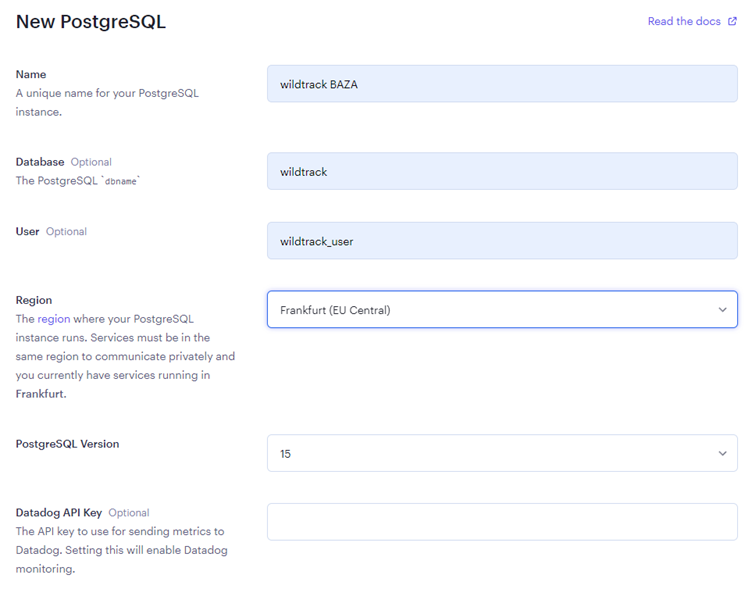
\includegraphics[scale=1]{slike/postavljanje baze1.png}
				\centering
				\caption{Stvaranje nove PostgreSQL baze}
				\label{fig:postavljanje baze1}
			\end{figure}

			 \item Dohvat podataka za spajanje
			 \begin{packed_item}
				\item Odabiremo \textit{Dashboard -  wildtrack BAZA -  Info}
				\item Spuštamo stranicu do izbora \textit{Connections} sa informacijama potrebnim za spajanje na bazu (slika \ref{fig:postavljanje baze2}).
			\end{packed_item}

			\begin{figure}[H]
				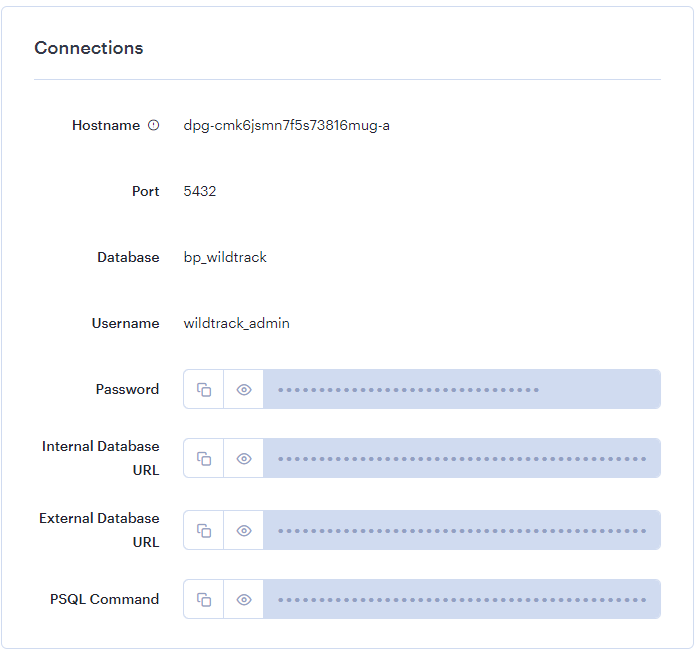
\includegraphics[scale=1]{slike/postavljanje baze2.png}
				\centering
				\caption{Dohvat podataka za spajanje baze}
				\label{fig:postavljanje baze2}
			\end{figure}

			\item Spajanje putem pgAdmina
			\begin{packed_item}
				\item Odabiremo \textit{Object - Create - Server}
				\item Na kartici \textit{General} unosimo ime servera kojeg otvaramo u pgAdminu
				\item Na kartici \textit{Connection} unosimo podatke kao na slici \ref{fig:postavljanje baze3} i spremamo ih sa \textit{Save}
			\end{packed_item}

			\begin{figure}[H]
				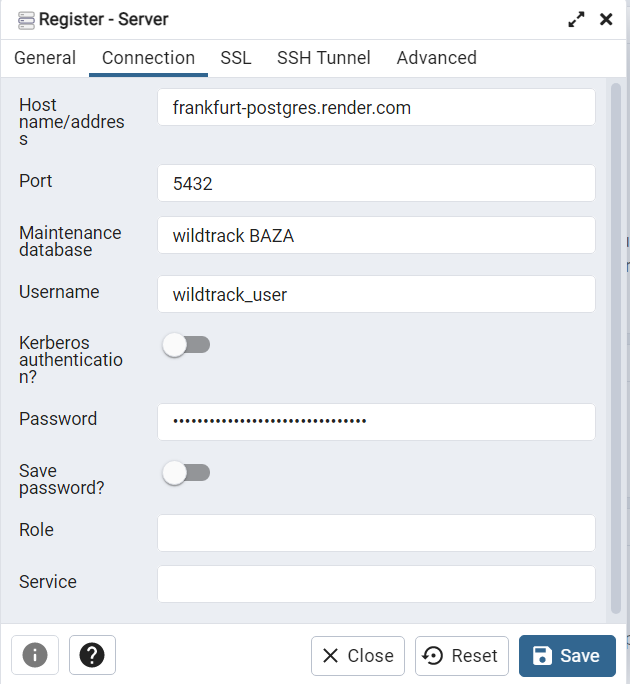
\includegraphics[scale=1]{slike/postavljanje baze3.png}
				\centering
				\caption{Unos podataka za spajanje baze}
				\label{fig:postavljanje baze3}
			\end{figure}

			\item Spajanje iz \textit{backenda}
			\begin{packed_item}
				\item U \textit{src/main/resources/application.properties} upisujemo naredbe sa slike \ref{fig:postavljanje baze4}
			\end{packed_item}
			
			\begin{figure}[H]
				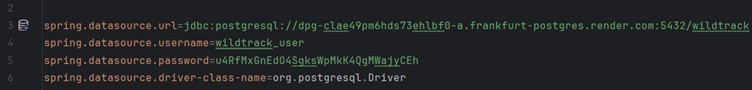
\includegraphics[scale=1]{slike/postavljanje baze4.png}
				\centering
				\caption{Spajanje baze iz \textit{backenda}}
				\label{fig:postavljanje baze4}
			\end{figure}


			\end{packed_enum}
			
			\eject 